\documentclass[12pt]{article}
\usepackage[utf8x]{inputenc}
\usepackage{amsmath}
\usepackage{multicol}
\usepackage{graphicx}
\usepackage{float}
\usepackage{dsfont}
\usepackage{textcomp}
\usepackage{amsfonts}
\usepackage{cleveref}
\usepackage{fancyhdr}
\setlength{\headheight}{14.5pt}
\renewcommand{\sectionmark}[1]{\markright{#1}{}}
\usepackage[T1]{fontenc}
\usepackage[colorinlistoftodos]{todonotes}
\usepackage[margin=2cm,a4paper]{geometry}
\newgeometry{left=2.0cm,right=2.0cm,top=2.5cm,bottom=2.5cm}
\usepackage{listings}
\setlength{\marginparwidth}{2cm}
\setlength{\parindent}{0pt}
\newcommand{\deriv}{\mathrm{d}}
\lstset{
    language=R,
    basicstyle=\scriptsize\ttfamily,
    commentstyle=\ttfamily\color{red},
    numbers=left,
    numbersty is le=\ttfamily\color{blue}\footnotesize,
    stepnumber=1,
    numbersep=5pt,
    backgroundcolor=\color{white},
    showspaces=false,
    showstringspaces=false,
    showtabs=false,
    frame=single,
    tabsize=2,
    captionpos=b,
    breaklines=true,
    breakatwhitespace=false,
    title=\lstname,
    escapeinside={},
    keywordstyle={},
    morekeywords={}
    }
\title{}
\pagestyle{fancy}
\fancyhf{}
\rhead{\leftmark}
\lhead{Exp.6 Rutherford Scattering}
\lfoot{PH520 Physics Laboratory A}
\rfoot{Page \thepage}
\renewcommand{\headrulewidth}{1pt}
\renewcommand{\footrulewidth}{1pt}
\begin{document}
\begin{titlepage}
\newgeometry{left=1.0in,right=1.0in,top=2.0in,bottom=2.0in}
\newcommand{\HRule}{\rule{\linewidth}{0.5mm}}
\begin{centering} 
%---------------------------------------------------------------------------
%	HEADING SECTIONS
%---------------------------------------------------------------------------

\includegraphics[scale=0.6]{Images/Uni_of_Kent.png}\\[1cm]
%---------------------------------------------------------------------------
%	TITLE SECTION
%---------------------------------------------------------------------------
\HRule \\[0.4cm]
\textsc{\large Astronomy, Space Science and Astrophysics}\\[0.5cm]
{ \Huge \bfseries Exp.6 Rutherford Scattering}\\[0.4cm]
\HRule \\[1.0cm]
%---------------------------------------------------------------------------
%	DATE SECTION
%---------------------------------------------------------------------------
\textsc{\Large PH520 - Stage 2}\\[0.5cm] 
\textsc{\Large Physics Laboratory A}\\[0.5cm] 
{\large Date: 11th Nov 2019 - 13th Jan 2020}\\[0.5cm]
%---------------------------------------------------------------------------
%	AUTHOR SECTION
%---------------------------------------------------------------------------
\begin{minipage}{0.625\textwidth}
\begin{center} \large
\emph{Report Author:} Lukasz R Tomaszewski \\[0.2cm]
\emph{Lab Partner:} Thomas O'Sullivan \\ [0.5cm]
{\large Word Count: 2397}\\
\end{center}
\end{minipage}\\[2cm]
\vfill
\end{centering} 
\end{titlepage}
%---------------------------------------------------------------------------
%	CONTENTS   
%---------------------------------------------------------------------------
\newpage
\begin{titlepage}
\begin{tableofcontents}
\end{tableofcontents}
\end{titlepage}
\newpage
%---------------------------------------------------------------------------
%	ABSTRACT
%---------------------------------------------------------------------------
\section{Abstract}
\label{Abstract Section}

By scattering $\alpha$-particles at different it’s proved Rutherford’s "scattering formula" \cref{Ruthe scat form} given an error of $\theta$=$\pm$1.5\textdegree. Shown in \cref{2.1.1 Graph} and \cref{2.1.2 Graph} a strong correlation within the data points relevant error margins is given between the experimental data and the theoretical data, this was done by valuing the coefficients A and B in \cref{Theory Eq} to be 0.00035 and 0.01 respectively. The experimental data was also corrected as the experiment measured values in a 2D horizontal plane whereas in fact it is a 3D cone, therefore a correction factor of $\sin(\theta)$ was deduced and multiplied with the experimentally $\alpha$ rate/s. The atomic number of aluminium and \cref{Atom Eq} proven by finding a strong correlated data angle i.e. -15\textdegree and its $\alpha$-particle Rate/s used in \cref{Atom Eq} to give a value of 12.88 which is just outside of the $\pm$0.1 error margin as the atomic number of aluminium is 13 \cite{CRC}. It was also proven that the ratio of Rate/s and the total number of $\alpha$-particles is physically dimensionless by associating the physical dimension with each parameters SI Units.

%---------------------------------------------------------------------------
%	INTRODUCTION
%---------------------------------------------------------------------------
\section{Introduction}
\label{Introduction Section}

"In 1911, Ernest Rutherford discovered the nucleus of the atom and kick started the age of nuclear physics. Since this, the Thompson model of the atom pioneered the understanding of the atom as it was discovered that the atom composed of very small electrons surrounded by a sea of positive charge to counter the electrons negative charge. Rutherford projected alpha particles at thin metal foils, while observing their deflection he noticed that the highly charged alpha particles went straight through the metal foils, where some scattered up to 180 degrees and a few deflected backwards, thus disproving the Thompson model. \cite{Exp.6-2019} \cite{Exp.6-Lab_book} \\

In this experiment, Rutherford's well known scattering experiment will be repeated as to find the following objectives: \cite{Exp.6-2019}
\begin{itemize}
    \item To record the direct count rate $N_d$ of $\alpha$-particles scattered by a gold foil as a function of the scattering angle $\theta$.
    \item To correct the count rates measured in one plane for the fact that the foil scatters in a 3D cone.
    \item To validate "Rutherford's scattering formula". 
    \item To determine the atomic number of aluminium experimentally. 
\end{itemize}

%---------------------------------------------------------------------------
%	METHODOLOGY
%---------------------------------------------------------------------------
\section{Methodology}
\label{Methodology Section}
%---------------------------------------------------------------------------
\subsection{Background}
\label{Background Subsection}

Within this experiment $\alpha$-particles collide with and penetrate a thin gold foil, at small angles a majority of the $\alpha$-particles scatter less than 1\textdegree, at large angles up to 180\textdegree only a few particle are scattered, this is called back scattering. With this observation, Rutherford formulated his "scattering formula":

\begin{equation}
N(\theta) = N_0 \hspace{0.1cm} c_f \hspace{0.1cm} d_f \hspace{0.1cm} \dfrac{Z^2 \hspace{0.1cm} e^4}{(8 \pi \hspace{0.1cm} \epsilon_0 \hspace{0.1cm} E_{\alpha})^2 \hspace{0.1cm} \sin^4(\theta / 2) }
\label{Ruthe scat form}
\end{equation} 

With the parameters set as:
\begin{multicols}{2}
    $N_0$ \hspace{0.1cm} Number of incident $\alpha$-particles \\
    $d_f$ \hspace{0.1cm} Foil thickness \\
    $E_{\alpha}$ \hspace{0.1cm} Energy of $\alpha$-particles \\
    $\epsilon_0$ \hspace{0.1cm} Dielectric constant (\cref{Useful Constants}) \\
    $c_f$ \hspace{0.1cm} Atomic concentration of foil \\
    $Z$ \hspace{0.1cm} Atomic number of the foil \\
    $e$ \hspace{0.1cm} elementary charge (\cref{Useful Constants}) \\
\end{multicols}
\vspace{0.5cm}

\begin{figure}[H]
\centering
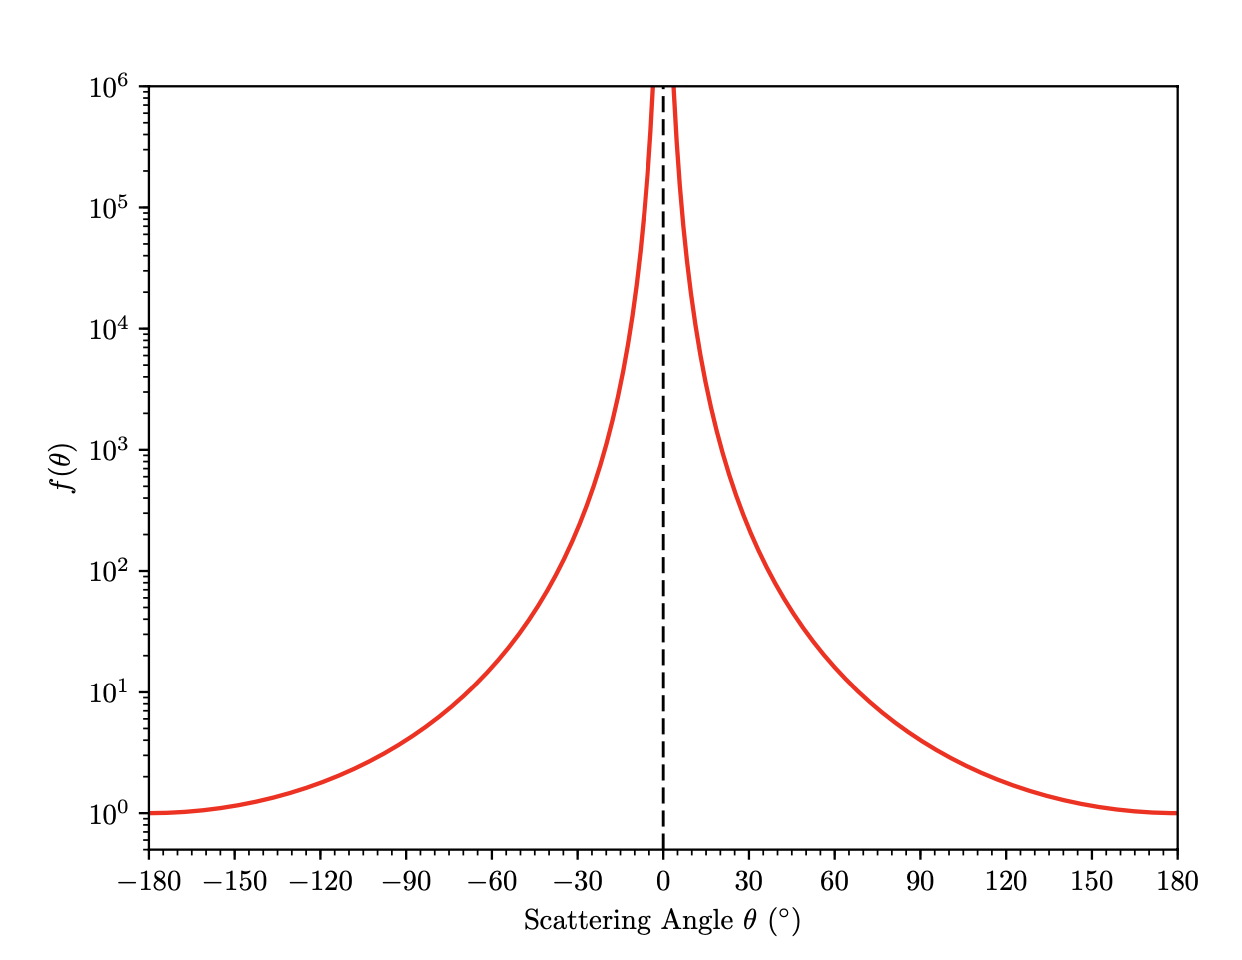
\includegraphics[scale=0.5]{Images/two.png}
\caption{Theoretical scattering rate as a function of angle \cref{SR Function}. From \cite{Exp.6-2019}.}
\label{Theoretical scattering rate as a function of angle}
\end{figure}

Rutherford's "scattering formula" can be simplified as the coefficients are constant, so the formula equates to the scattering of the scattering of $\alpha$-particles as a function of angle: 

\begin{equation}
f(\theta) = \dfrac{1}{\sin^4(\theta / 2)}
\label{SR Function}
\end{equation} 

As f($\theta$) tends to infinity as a singularity occurs as the angle approaches very small angles, this can be view by graphical representation in \cref{Theoretical scattering rate as a function of angle}. Due to this, the experimental data recorded will only be compared to the theoretical data of angles |$\theta$|$\leq$ $\pm$5\textdegree, on the other hand its clear that the scattering rate become very small at larger angles therefore a limit is set to |$\theta$|$\leq$ $\pm$30\textdegree. These limits ensure a significant amount of high quality experimental data so that it can be compared theoretically. \\

By being able to change the gold foil with aluminium foil and by keeping the induced angle the same the atomic number of aluminium can be computed, by using the scattering angles:

\begin{equation}
\dfrac{N_{Au}}{N_{A1}} = \dfrac{c_{Au} \hspace{0.1cm} d_{Au} \hspace{0.1cm} {Z_{Au}}^2}{c_{A1} \hspace{0.1cm} d_{A1} \hspace{0.1cm} {Z_{A1}}^2}
\label{Atom Eq}
\end{equation} 

With the parameters set as:
\begin{multicols}{2}
    $N_{Au}$ \hspace{0.1cm} Scattering rate of gold \\
    $c_{Au}$ \hspace{0.1cm} Atomic concentration of gold \\
    $d_{Au}$ \hspace{0.1cm} Foil thickness of gold \\
    $Z_{Au}$ \hspace{0.1cm} Atomic number of gold \\
    $N_{A1}$ \hspace{0.1cm} Scattering rate of aluminium \\
    $c_{A1}$ \hspace{0.1cm} Atomic concentration of aluminium \\
    $d_{A1}$ \hspace{0.1cm} Foil thickness of aluminium \\
    $Z_{A1}$ \hspace{0.1cm} Atomic number of aluminum 
\end{multicols}
\vspace{0.5cm}

%---------------------------------------------------------------------------
\subsection{Experimental Setup}
\label{Experimental Setup Subsection}
%---------------------------------------------------------------------------
\subsubsection{Recording the scattering rate as a function of angle}
\label{Recording the scattering rate as a function of angle Subsubsection}

\begin{figure}[H]
\centering
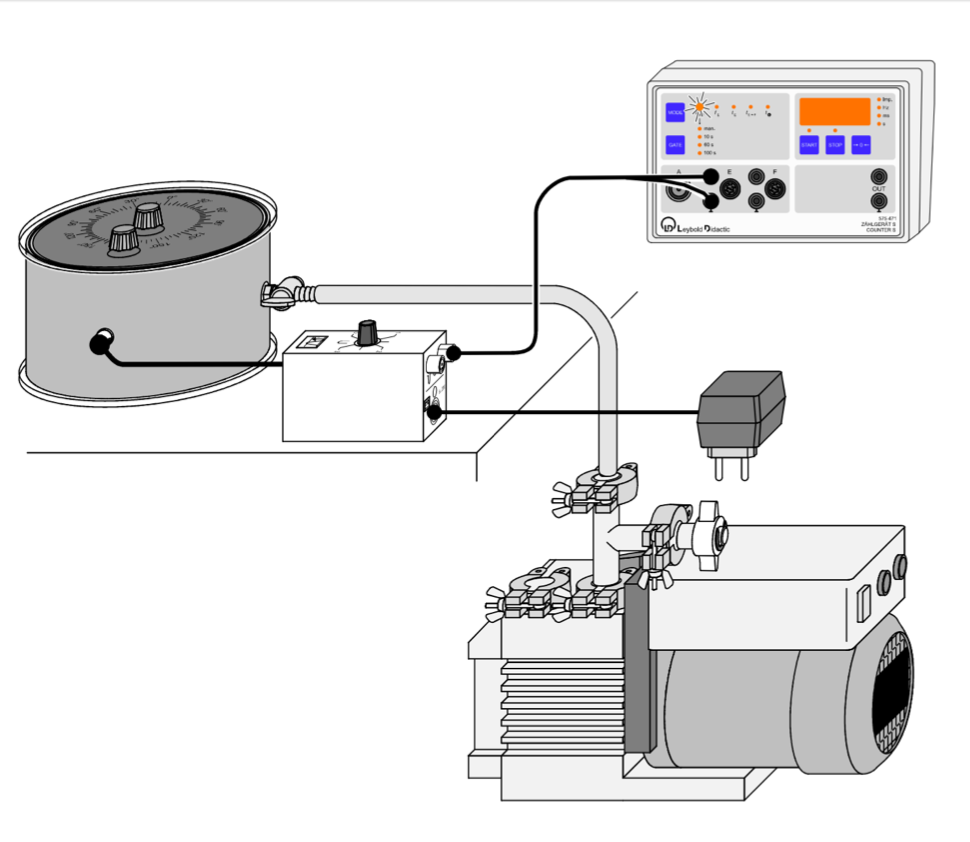
\includegraphics[scale=0.5]{Images/three.png}
\caption{Setup of apparatus. From \cite{Exp.6-2019}\cite{Two}.}
\label{Setup of Apparatus}
\end{figure}

By setting up the apparatus depicted in \cref{Setup of Apparatus}, the vacuum within the chamber is created by using the vacuum pump to extract the air, thus improving the quality of the experiment so that the $\alpha$-particles aren't affected by the air molecules when being fired at the gold foil. Inside the chamber the $\alpha$-particles are fired form an Am-241 source, through a 5mm wide slit in front of the gold foil and thus scattered, by changing the angle of the detector on the other side of the foil, the scattering rate as a function of the angle can be observed. The detector measures how many $\alpha$-particles it detects and feeds the data through a discriminator preamplifier so that the data can organised and any external "noise" discarded, the quality data shows onto a piece of computer software called CASSY. Within this program the "gate time" can be inputted which collects data per the specified gate time (counts per second) thus collating the results so that the number of $\alpha$particles can be divided by the gate time to give rate per second, this allows more control on the quality of the data sourced. \\

\begin{multicols}{2}
\begin{figure}[H]
\centering
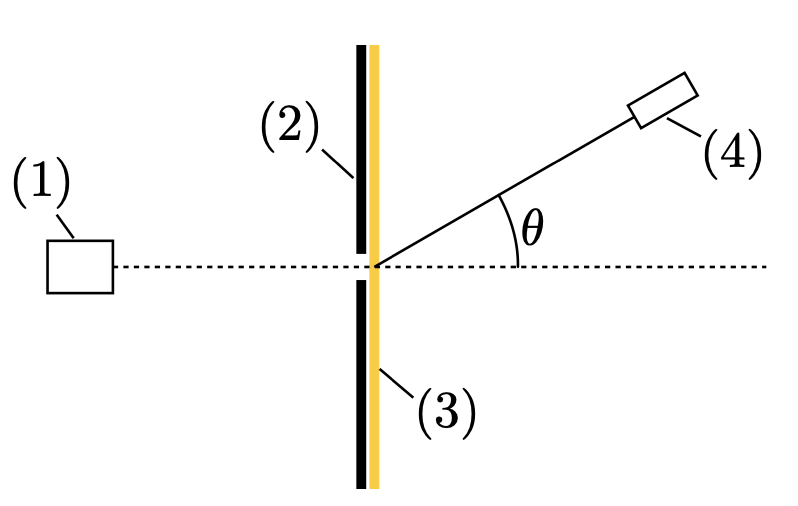
\includegraphics[scale=0.5]{Images/four.png}
\caption{Inside the chamber. From \cite{Exp.6-2019}\cite{Two}.}
\label{Inside the chamber}
\end{figure}


(1) = Am-241 source \\
(2) = 5mm/1mm slit \\
(3) = Gold/ Aluminium foil \\
(4) = Detector
\end{multicols}

Setting the discriminator preamplifier to -0.2v at the start of the experiment tills the counts per seconds holds steady (falls to zero), this in effect gives a zero point to which the detector collects the data. By turning the angle of the detector by $\pm$5\textdegree shown in \cref{Inside the chamber}, the program can start and measurements are taken over every 10 seconds for 60 seconds. This allows the experiment to be unbiased as the time is unchanged. Increasing the angle from $\pm$5\textdegree and recording the amount of scattered $\alpha$-particles until $\pm$30\textdegree is reached. The total amount of particles are then averaged then divided by the gate time to give $\alpha$-particle rate per second. \\

Further exploring this, increasing the gate time to 30 seconds, but instead of keeping the total elapsed time the same, en-devouring to allow more than a total of 100+ particles to be detected over the elapsed time to reduce statistical error when calculating the rate per second.

%---------------------------------------------------------------------------
\subsubsection{Measuring the atomic number of Aluminium}
\label{Measuring the atomic number of Aluminium Subsubsection}

By changing the 5mm slit with a 1mm slit (\cref{Inside the chamber}) to give a smaller target area for the $\alpha$-particles to collide with the foil, the foil is also changeable so that measurements for the rate of particles scattered is obtained for both gold and aluminium foils. Instead of utilizing a large difference in angle as before with the limits being $\pm$5\textdegree \hspace{0.1mm} $\geq$ |$\theta$| $\leq$ $\pm$30\textdegree, a suitable angle with a reasonable count rate such as -15\textdegree will be used for both types of foils when using the scattering rates of both materials in \cref{Atom Eq} when calculating the atomic number of aluminium. The measurements can be repeated for other angles such as -10\textdegree, -5\textdegree and +5\textdegree to validate and compare the value of the atomic number of aluminium with each angle. \\


%---------------------------------------------------------------------------
\subsection{Evaluation \& Results}
\label{Evaluation & Results Subsection}

%---------------------------------------------------------------------------
\subsubsection{Recording the scattering rate as a function of angle}
\label{3.3 Recording the scattering rate as a function of angle Subsubsection}

When the $\alpha$-particles are fired from the Am-241 source and passes through the 1mm/5mm slit the $\alpha$-particles scatter only in a horizontal plane due to the shape of the slit, whereas in the theoretical data is scattered in a 3D cone as seen in \cref{3D Cone}. Due to this a mathematical correction must be applied to the experimental data to compare with the theoretical data. \\

\begin{figure}[H]
\centering
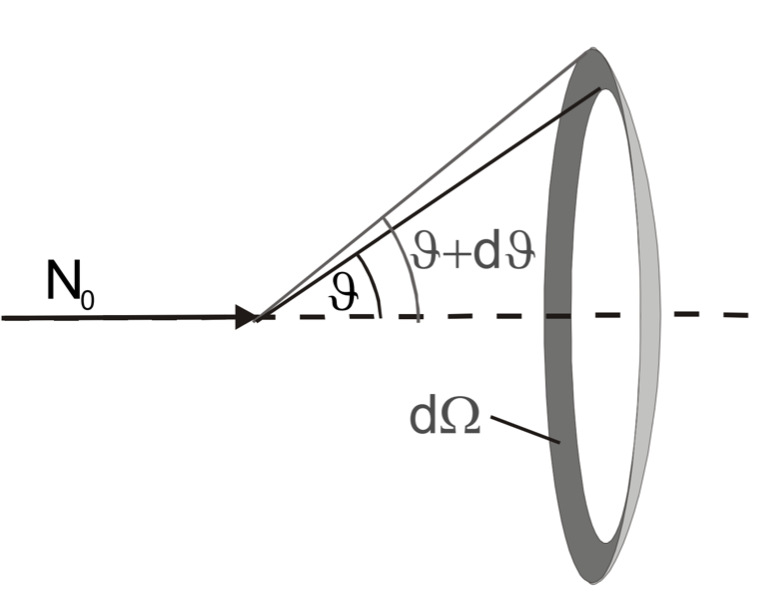
\includegraphics[scale=0.5]{Images/six.png}
\caption{$\alpha$-particles scattering into a 3D cone. From \cite{Exp.6-2019}\cite{Two}.}
\label{3D Cone}
\end{figure}

This correction is calculated as follows; \\

If the end of the cone in laid flat into rectangular strip (area in grey in \cref{3D Cone}) and say the diameter equals to 'h' then the area of the end and the circle can be determined; 

\begin{equation}
A_A = 2\pi r h
\end{equation}

\begin{equation}
A_d = \pi r^2 \rightarrow \pi {(h/2)}^2 \rightarrow \dfrac{\pi h^2}{4}
\end{equation}

\begin{equation}
\dfrac{A_A}{A_d} = \dfrac{2 \pi r h}{(\pi h^2)/4} \rightarrow \dfrac{8r}{h}
\end{equation}
\vspace{0.2cm}

By changing this equation into 3D polar coordinates as the $alpha$-particles scatter into a circle, r now becomes $r = \sin \theta$. This correction factor is then multiplied by the experimental data fit the theoretical curve of;

\begin{equation}
f(\theta) = \dfrac{A}{\sin^4((\theta - B)/2)}
\label{Theory Eq}
\end{equation}
\vspace{0.2cm}

Where A and B are coefficients that represents the vertical shift and horizontal drift respectively of the theoretical curve. These coefficients are to be altered to align itself with the experimental data so that a true comparison can be made and any and all visible discrepancies of the experimental data can been recorded. \\

%---------------------------------------------------------------------------
\subsubsection{Determining the atomic number of aluminium}
\label{3.3 Determining the atomic number of aluminium Subsubsection}

To determine the atomic number of aluminium, rearrange \cref{Atom Eq} to find $Z_{A1}$;

\begin{equation}
\dfrac{N_{Au}}{N_{A1}} = \dfrac{c_{Au} \hspace{0.1cm} d_{Au} \hspace{0.1cm} {Z_{Au}}^2}{c_{A1} \hspace{0.1cm} d_{A1} \hspace{0.1cm} {Z_{A1}}^2} \rightarrow
{Z_{A1}} = \sqrt{\dfrac{N_{A1} \hspace{0.1cm} c_{Au} \hspace{0.1cm} d_{Au} \hspace{0.1cm} {Z_{Au}}^2}{N_{Au} \hspace{0.1cm} c_{A1} \hspace{0.1cm} d_{A1}}}
\end{equation} 
\vspace{0.2cm}

$Z_{Au}$ is known in \cref{Useful Constants}, the scattering rates $Z_{Au}$ and $Z_{A1}$ are found in the experimental data then corrected with the correction factor. The atomic concentration needs to be calculated via;

\begin{equation}
c = \dfrac{Mass Density}{Atomic Weight} \times Avogadro's Constant
\end{equation}

Thus filling the parameters with their values will calculate an approximated value for the atomic number of aluminium.

%---------------------------------------------------------------------------
\subsection{Error Analysis}
\label{Error Analysis Subsection}

The errors throughout this experiment there are 3 main errors to consider and   are the same throughout, though using computer software where errors are fairly accurate, it still produces a margin for error though very small. 

\begin{table}[H]
\begin{center}
 \begin{math}
 \begin{tabular}{c c c}
 Angle ($\theta$)  = & $\pm$1.5\textdegree \\
 Time (s) = & $\pm$0.1s \\
 $Na_1$ = & $\pm$1 \\
 \end{tabular}
 \end{math}
 \caption{Error Analysis.}
 \label{Error Analysis}
\end{center}
\end{table}

\textbf{\underline{Standard Error for section 2.1.1 in \cite{Exp.6-2019}}}:

\begin{equation}
\sigma = \sqrt{\dfrac{1}{N} \sum_{i=1}^{N}(x_i - \Bar{x})^2}
\end{equation}

\begin{equation}
\sigma = 174.88
\end{equation}

\textbf{\underline{Standard Error for section 2.1.2 in \cite{Exp.6-2019}}}:

\begin{equation}
\sigma = \sqrt{\dfrac{1}{N} \sum_{i=1}^{N}(x_i - \Bar{x})^2}
\end{equation}

\begin{equation}
\sigma = 3397.22
\end{equation}

\textbf{\underline{Standard Error for section 2.2 in \cite{Exp.6-2019}}}:

\begin{equation}
\sigma = \sqrt{\dfrac{1}{N} \sum_{i=1}^{N}(x_i - \Bar{x})^2}
\end{equation}

\begin{equation}
{\sigma}_{Au} = 2508.17 \\
{\sigma}_{A1} = 1876.23
\end{equation}

%---------------------------------------------------------------------------
%	REPORT & FINDINGS
%---------------------------------------------------------------------------
\section{Results \& Findings}
\label{Results & Findings Section}
%---------------------------------------------------------------------------
\subsection{Recording scattering rate as a function of angle}
\label{Recording scattering rate as a function of angle Findings}

When applying the correction factor of $\sin(\theta)$ and determining the theoretical data (\cref{Theory Eq}), the value for $\theta$ is in radians;

\begin{table}[H]
\begin{center}
 \footnotesize
 \begin{tabular}{|c||c|c|c|c|c|c||c|c|c|c|c|c|}
 \hline
 \multicolumn{13}{|c|}{Converting angles into radians} \\
 \hline \hline
 $\theta$ & -30 & -25 & -20 & -15 & -10 & -5 & +5 & +10 & +15 & +20 & +25 & +30 \\
 \hline
 Radians & -0.52 & -0.44 & -0.35 & -0.26 & -0.17 & -0.09 & 0.09 & 0.17 & 0.26 & 0.35 & 0.44 & 0.52 \\
 \hline
 \end{tabular} \\ 
 \caption{Angles into Radians}
 \label{Angles into Radians}
\end{center}
\end{table}

By obtaining the experimental results from \cref{Rate of particles within a gate time of 10s over 60s table}, the correction factor can be applied and the theoretical data derived from \cref{Evaluation & Results Subsection}. A correlation can be seen with in the limits specified in \cref{Background Subsection}, proving that as $\theta$ tends to zero the rate of scattering increases. The theoretical data coefficients in \cref{Theory Eq} were proven to equal A = 0.00035 and B = 0.01. \\

\begin{figure}[H]
\centering
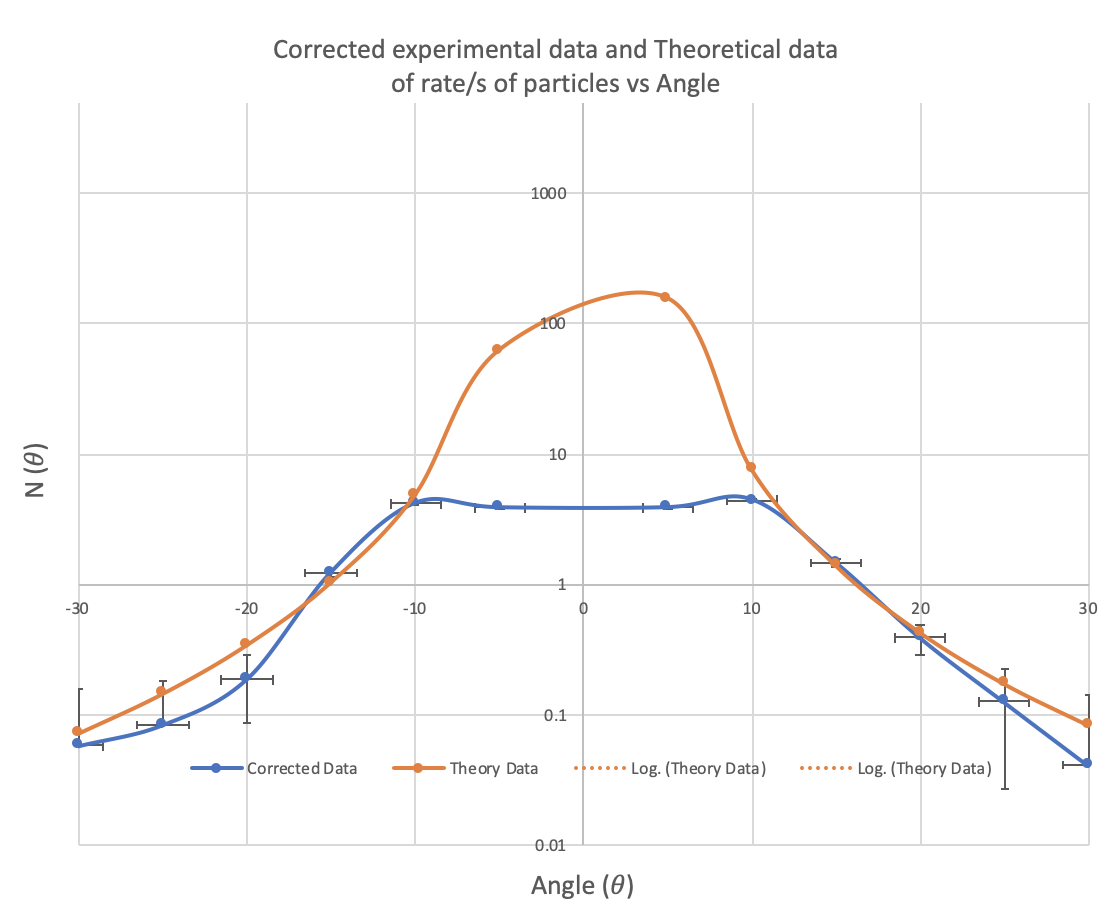
\includegraphics[scale=0.7]{Images/211.png}
\caption{Corrected experimental and theoretical data of $rate/s$ vs angle withing a gate time of 10s over 60s. From (\cref{Rate of particles within a gate time of 10s over 60s table}).}
\label{2.1.1 Graph}
\end{figure}

\begin{table}[H]
\begin{center}
 \footnotesize
 \begin{tabular}{|c||c|c|c|c|c|c||c|c|c|c|c|c|}
 \hline
 \multicolumn{13}{|c|}{Rate of particles entering the chamber within a gate time of 10s over 60s} \\
 \hline \hline
 $\theta$ & -30 & -25 & -20 & -15 & -10 & -5 & +5 & +10 & +15 & +20 & +25 & +30 \\
 \hline
 \hline
 Time (s) & 60.0 & 60.0 & 60.0 & 60.0 & 60.0 & 60.0 & 60.0 & 60.0 & 60.0 & 60.0 & 60.0 & 60.0 \\
 \hline
 *Avg.$Na_1$ & 1.17 & 2.00 & 5.50 & 47.67 & 241.17 & 446.17 & 447.00 & 257.67 & 57.00 & 11.50 & 3.00 & 0.08 \\
 \hline
 *$Rate/s$ & 0.12 & 0.20 & 0.55 & 4.77 & 24.12 & 44.62 & 44.70 & 25.77 & 5.70 & 1.15 & 0.30 & 0.08 \\
 \hline \hline
 *$C-Rate/s$ & 0.06 & 0.08 & 0.19 & 1.23 & 4.19 & 3.89 & 3.90 & 4.47 & 1.48 & 0.39 & 0.13 & 0.04 \\
 \hline
 *$T-Rate/s$ & 0.08 & 0.15 & 0.33 & 0.90 & 3.51 & 28.61 & 1301.50 & 21.26 & 2.93 & 0.79 & 0.30 & 0.14 \\
 \hline
 \end{tabular} \\ [0.2cm]
 *Avg.$Na_1$ = Average number of particle in time (s). \\
 *$Rate/s$ = Rate of particles per second. \\
 *$C-Rate/s$ = Corrected rate of particles per second. \\
 *$T-Rate/s$ = Theoretical rate of particles per second.
 \caption{Rate of particles within a gate time of 10s over 60s}
 \label{Rate of particles within a gate time of 10s over 60s table}
\end{center}
\end{table}

From \cref{2.1.1 Graph} the experimental data correlates with the theoretical data, it can be seen that between +20\textdegree and +10\textdegree both sets of data match, with some variations in the comparison in the negative axis. But apart from -20\textdegree all the experimental data points are within their individual error margin with the theoretical data. These results were attained by keeping the overall time fixed with fluctuating amount of particles, on the other hand while making sure 100+ $\alpha$-particles were detected and total time is the variable.  \\

\begin{figure}[H]
\centering
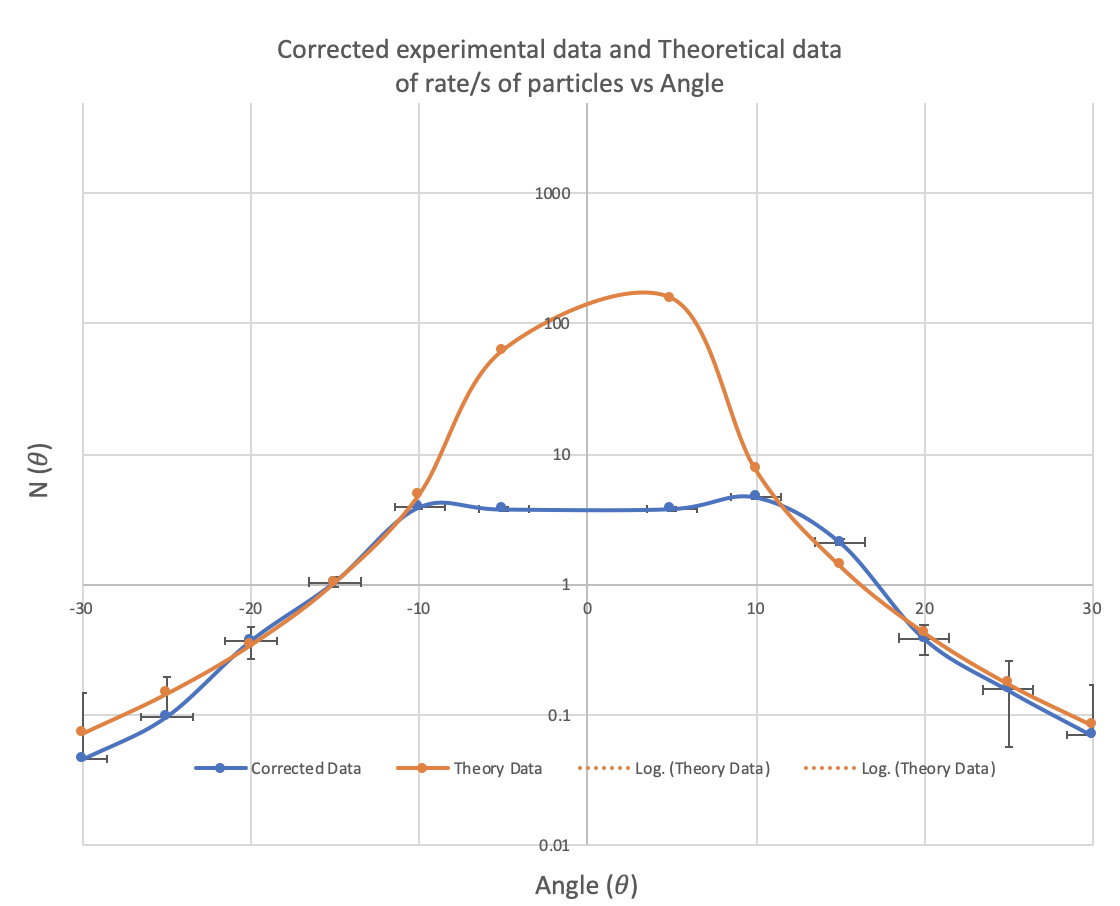
\includegraphics[scale=0.7]{Images/212.png}
\caption{Corrected experimental and theoretical data of $rate/s$ vs angle withing a gate time of 40s ensuring 100+ particles. From (\cref{Rate of particles within a gate time of 40s ensuring 100+ particles table}}
\label{2.1.2 Graph}
\end{figure}

\begin{table}[H]
\begin{center}
 \footnotesize
 \begin{tabular}{|c||c|c|c|c|c|c||c|c|c|c|c|c|}
 \hline
 \multicolumn{13}{|c|}{Rate of particles entering the chamber within a gate time of 40s ensuring 100+ particles} \\
 \hline \hline
 $\theta$ & -30 & -25 & -20 & -15 & -10 & -5 & +5 & +10 & +15 & +20 & +25 & +30 \\
 \hline \hline
 Time (s) & 1120.8 & 480.3 & 200.1 & 200.1 & 200.1 & 200.1 & 200.1 & 200.1 & 200.1 & 200.1 & 280.2 & 840.6\\
 \hline
 *Total $Na_1$ & 103 & 111 & 217 & 812 & 4518 & 8703 & 8762 & 5402 & 1648 & 229 & 104 & 118 \\
 \hline
 *$Rate/s$ & 0.09 & 0.23 & 1.09 & 4.060 & 22.59 & 43.52 & 43.81 & 27.01 & 8.24 & 1.15 & 0.37 & 0.14 \\
 \hline \hline
 *$C-Rate/s$ & 0.05 & 0.10 & 0.37 & 1.05 & 3.92 & 3.79 & 3.82 & 4.69 & 2.13 & 0.39 & 0.16 & 0.07  \\
 \hline
 *$T-Rate/s$ & 0.08 & 0.15 & 0.33 & 0.90 & 3.51 & 28.61 & 1301.50 & 21.26 & 2.93 & 0.79 & 0.30 & 0.14 \\
 \hline
 \end{tabular} \\ [0.2cm]
 *Avg.$Na_1$ = Average number of particle in time (s). \\
 *$Rate/s$ = Rate of particles per second. \\
 *$C-Rate/s$ = Corrected rate of particles per second. \\
 *$T-Rate/s$ = Theoretical rate of particles per second.
 \caption{Rate of particles within a gate time of 40s ensuring 100+ particles}
 \label{Rate of particles within a gate time of 40s ensuring 100+ particles table}
\end{center}
\end{table}

By allowing at least 100+ $\alpha$-particles to be detected and allowing the total time to fluctuate the correlation in \cref{2.1.2 Graph} the mirror image to \cref{2.1.2 Graph}. While the negative axis shows a strong relationship between the angles -20\textdegree to -10\textdegree, the positive doesn't show the same relationship as in \cref{2.1.1 Graph} instead a relationship between +20\textdegree to +30\textdegree emerges. \\

This part of the experiment shows more correlation to the theoretical data than in \cref{2.1.1 Graph}, this is mostly due to allowing more particles enter the chamber and be scattered instead of the total time being fixed. The gate time was also increased to 40 seconds instead of 10 seconds to allow more $\alpha$-particle to be detected, by increasing the gate time also increase the average amount of $\alpha$-particles though irrelevant as the average number of $\alpha$-particles are divided by their gate time, giving rate per second. \\

\subsection{Measuring the atomic number of Aluminium}
\label{Measuring the atomic number of Aluminium Findings}

\begin{table}[H]
\begin{center}
 \footnotesize
 \begin{tabular}{|c||c|c|c|c||c|c|c|c||c|}
 \hline
 \multicolumn{10}{|c|}{Rate of particles within a gate time of 30s of both Gold \& Aluminium foils} \\
 \hline \hline
 Material & \multicolumn{4}{c||}{Aluminium Foil} & \multicolumn{4}{c||}{Gold Foil} & \multicolumn{1}{|c|}{} \\
 \hline 
 $\theta$ & -15 & -10 & -5 & +5 & -15 & -10 & -5 & +5 & Error \\
 \hline
 \hline
 Time (s) & 600.2 & 300.2 & 300.2 & 300.2 & 300.2 & 300.2 & 300.2 & 300.2 & $\pm0.1s$ \\
 \hline
 *Total $Na_1$ & 13 & 29 & 816 & 5246 & 70 & 338 & 1872 & 4160 & $\pm1.0$ \\
 \hline
 *$Rate/s$ & 0.022 & 0.097 & 2.720 & 17.487 & 0.233 & 1.127 & 6.240 & 13.867 & $\pm1.0s$ \\
 \hline \hline
 *$C-Rate/s$ & 0.036 & 0.106 & 1.489 & 9.576 & 0.379 & 1.229 & 3.417 & 7.594 & $\pm1.0s$ \\
 \hline
 \end{tabular} \\ [0.2cm]
 *Total $Na_1$ = Total number of particles in the chamber in time (s). \\
 *$Rate/s$ = Rate of particles entering the chamber per second. \\
 *$C-Rate/s$ = Corrected rate of particles entering the chamber per second.
 \caption{Rate of particles on Gold \& Aluminium foils}
 \label{2.2 Results}
\end{center}
\end{table}

By observing the difference of $\alpha$-particle detected through the aluminium foil the at angles -15\textdegree and -10\textdegree are significantly less than its golden counter-part. This is due to the fact the larger the angle the closer the $\alpha$-particle gets to striking the aluminium nuclei, which has happened here. This observation can make use of using the scattering angle to determine the materials nuclei diameter. \\

There are still two parameter that need to be calculated, the atomic concentration of the gold and aluminium foils, using \cite{CRC}:  \\

\begin{equation}
{c} = \dfrac{Mass density}{Atomic Weight} \times Avogadro's Constant
\end{equation} 
\vspace{0.2cm}

\begin{multicols}{2}
$Md_{Au}$ = 0.193 $g/m^3$ \\
$Aw_{Au}$ = 196.966569 kg \\
$Md_{A1}$ = 0.027 $g/m^3$ \\
Avogadros Constant = ${6.022_{x10}}^{23}$ $mol^{-1}$  \\
$Aw_{A1}$ = 26.9815386 

\end{multicols}

\textbf{\underline{Gold}}: \\

\begin{equation}
{c} = \dfrac{0.193}{196.966569} \times {6.022_{x10}}^{23} = {5.9_{x10}}^{20} mol/m^3
\end{equation} 

\textbf{\underline{Aluminium}}: \\

\begin{equation}
{c} = \dfrac{0.0270}{26.9815386} \times {6.022_{x10}}^{23} = {6.02_{x10}}^{20} mol/m^3
\end{equation} 
\vspace{0.1cm}

\textbf{\underline{Atomic number of Aluminum}}: \\

\begin{equation}
{Z_{A1}} = \sqrt{\dfrac{N_{A1} \hspace{0.1cm} c_{Au} \hspace{0.1cm} d_{Au} \hspace{0.1cm} {Z_{Au}}^2}{N_{Au} \hspace{0.1cm} c_{A1} \hspace{0.1cm} d_{A1}}}
\label{Atom Ali}
\end{equation} 

With the parameters set as:
\begin{multicols}{2}
    $N_{Au}$ \hspace{0.1cm} Scattering rate of gold = (\cref{2.2 Results})\\
    $c_{Au}$ \hspace{0.1cm} Atomic concentration of gold = ${5.9_{10}}^{20}$ $mol/m^3$\\
    $d_{Au}$ \hspace{0.1cm} Foil thickness of gold = ${2_{x10}}^{-6}$m \cite{Exp.6-2019} \\
    $Z_{Au}$ \hspace{0.1cm} Atomic number of gold = 79 (\cref{Useful Constants})\\
    $N_{A1}$ \hspace{0.1cm} Scattering rate of aluminium = (\cref{2.2 Results}) \\
    $c_{A1}$ \hspace{0.1cm} Atomic concentration of aluminium = ${6.02_{10}}^{20}$ $mol/m^3$ \\
    $d_{A1}$ \hspace{0.1cm} Foil thickness of aluminium = ${7_{x10}}^{-6}$m \cite{Exp.6-2019} \\
    $Z_{A1}$ \hspace{0.1cm} Atomic number of aluminum = ? 
\end{multicols}
\vspace{0.5cm}

By applying the corrected scattering rates of the Aluminium and Gold foils to \cref{Atom Ali} we get:

\begin{equation}
{Z_{Au}} (\theta = -15) = \sqrt{\dfrac{0.036 \times 5.9_{\times10^{20}} \times 2_{\times10^{-6}} \times 79^2}{0.379 \times 6.02_{\times10^{20}} \times 7_{\times10^{-6}}}} = 12.88
\end{equation} 

\begin{equation}
{Z_{Au}} (\theta = -10) = \sqrt{\dfrac{0.106 \times 5.9_{\times10^{20}} \times 2_{\times10^{-6}} \times 79^2}{1.229 \times 6.02_{\times10^{20}} \times 7_{\times10^{-6}}}} = 12.28
\end{equation} 

\begin{equation}
{Z_{Au}} (\theta = -5) = \sqrt{\dfrac{1.489 \times 5.9_{\times10^{20}} \times 2_{\times10^{-6}} \times 79^2}{3.417 \times 6.02_{\times10^{20}} \times 7_{\times10^{-6}}}} = 27.60
\end{equation} 

\begin{equation}
{Z_{Au}} (\theta = +5) = \sqrt{\dfrac{9.576 \times 5.9_{\times10^{20}} \times 2_{\times10^{-6}} \times 79^2}{7.594 \times 6.02_{\times10^{20}} \times 7_{\times10^{-6}}}} = 46.94
\end{equation} 
\vspace{0.2cm}

The atomic number of Aluminium had the value 13 \cite{CRC}, as can been seen for the larger angles -15\textdegree and -10\textdegree the values ascertained by \cref{Atom Ali} are fairly accurate more so for -15\textdegree as it had a stable $\alpha$-particle count but for the smaller angle -5\textdegree and +5\textdegree as hypothesised in \cref{Background Subsection}, 0\textdegree tends to infinity due to a singularity occurring. 

\subsection{Question}
\label{Question Findings}

The question in \cite{Exp.6-2019} states; \\

\begin{centering}
"In \cref{Ruthe scat form} the ratio $\dfrac{N(\theta)}{N_0}$ should be dimensionless; show this?" \\
\end{centering}
\vspace{0.5cm}

By utilizing each parameters individual SI units, their dimensions can be sourced. Simplifying Rutherford scattering formula \cref{Ruthe scat form} into 
\cref{simple} by removing all the constant with no SI units. The dimensions for each associated SI unit is sourced \cite{CRC} and shown in \cref{Dimensions Nomenclature}.

\begin{multicols}{2}
\centering

\begin{equation}
N(\theta) = N_0 \hspace{0.1cm} c_f \hspace{0.1cm} d_f \hspace{0.1cm} \dfrac{Z^2 \hspace{0.1cm} e^4}{(8 \pi \hspace{0.1cm} \epsilon_0 \hspace{0.1cm} E_{\alpha})^2 \hspace{0.1cm} \sin^4(\theta / 2) }
\end{equation} 

\begin{equation}
\dfrac{N\theta}{N_0} = \dfrac{Z^2 \hspace{0.1cm} C_f \hspace{0.1cm} d_f \hspace{0.1cm} e^4}{(8\pi \hspace{0.1cm} \epsilon_0 \hspace{0.1cm} E_{\alpha})^2}
\end{equation} 

\begin{equation}
\dfrac{N\theta}{N_0} = \dfrac{C_f \hspace{0.1cm} d_f \hspace{0.1cm} e^4}{\epsilon_0^2 \hspace{0.1cm} E_{\alpha}^2}
\label{simple}
\end{equation} 

\begin{table}[H]
\begin{center}
 \footnotesize
 \begin{tabular}{c c c}
 \textbf{\underline{Nomenclature}}; \\ [0.3cm]
 Symbol & SI Unit & Dimension \\
 \hline \\ [-0.3cm]
 $C_f$ & $M^{-3}$ & $L^{-3}$ \\[0.05cm]
 $d_f$ & $M$ & $L$ \\[0.05cm]
 $e$ & $C$ & $IT$ \\[0.05cm]
 $e^4$ & $C^4$ & $I^4T^4$ \\[0.03cm]
 $\epsilon_0$ & $C^2 / NM^2$ & $(IT)^2 / MLT^{-2}L^2$ \\[0.09cm]
 $\epsilon_0^2$ & $C^4 / N^2M^4$ & $I^4T^4 / M^2L^2T^{-4}L^4$ \\[0.09cm]
 $E_{\alpha}$ & $J$ & $ML^2T^{-2}$ \\[0.09cm]
 $E_{\alpha}^2$ & $J^2$ & $M^2L^4T^{-4}$ \\
 \end{tabular}
 \caption{Dimensions Nomenclature}
 \label{Dimensions Nomenclature}
\end{center}
\end{table}
\end{multicols}

\vspace{0.5cm}

Thus by trading the SI units for the associated dimensions in \cref{simple}, the dimensions cancel out and show that the ratio is truly dimensionless. \\ 

\begin{equation}
\dfrac{N\theta}{N_0} = \dfrac{(L^{-3})(L)(I^4T^4)}{(I^4T^4 / M^2L^2T^{-4}L^4)(M^2L^4T^{-4})} = \dfrac{L^{-2} I^4 T^4}{(I^{4}T^{4}M^{-2}L^{-2}T^{4}L^{-4})(M^2L^4T^{-4})}
\end{equation}

\begin{equation}
\dfrac{N\theta}{N_0} = \dfrac{(L^{-2}I^4T^4)(T^4 L^4 M^2)}{(I^{4}T^{4}L^{-2}T^{4})(M^2L^4)} = \dfrac{T^8 I^4 L^2 M^2}{T^8 I^4 L^2 M^2} = 0
\end{equation}

%---------------------------------------------------------------------------
%	DISCUSSION
%---------------------------------------------------------------------------
\section{Discussion}
\label{Disscussion Section}

The only variable error in this experiment was affecting the vacuum or detector, though these were prevented by not moving the detector only when changing the angle and not moving or removing the lid/ pipes of the vacuum chamber the small possibility of error could be to blame for the deviation of results between the experimental and theoretical data. This experiment was completed in 3 separate 2hr intervals thus the vacuum was destroyed and made live twice as well as the detector could have been hit thus affected its performance, this is taken into account as an error that affected the results as the experiments apparatus was not fair, this could've been avoided by completing the entire experiment in one session, thus not affecting or changing the apparatus. \\



%---------------------------------------------------------------------------
%	CONCLUSION
%---------------------------------------------------------------------------
\section{Conclusion}
\label{Conclusion Section}

Rutherford's scattering formula was proved as it was compared to physically collected experimental data which is corrected to account for the 3-dimensional cone scattering of the $\alpha$-particles. \cref{2.1.2 Graph} shows a strong correlation as a total of 100+ $\alpha$-particles were detected giving stronger quality results. But in both \cref{2.1.1 Graph} and \cref{2.1.2 Graph} shows a relationship between both sets of data at $\pm$15\textdegree clearly indicates an angle where reasonable results occur, this observation foreshadowed using 15\textdegree to determine the atomic number of aluminium. \\

By determining a positive relationship with the experimental and theoretical data with the angle -15\textdegree, this angle was used as the reference point for which its rate/s was used to accurately prove \cref{Atom Eq}. Not only prove \cref{Atom Eq} but prove the hypothesis \cref{Background Subsection}, the closer $\theta$ = 0, a singularity occurs and the results become unstable. Therefore the angles -5\textdegree and +5\textdegree were dismissed, with -10\textdegree forming a value of 12 instead of -15\textdegree giving 13, which is the atomic number of aluminium \cite{CRC}. While recording these results it was obvious to see by the difference of the count rate of $\alpha$-particles per angle between both the aluminium and gold foils that the size of the nucleus can be determined by using the scattering angle.

%---------------------------------------------------------------------------
%	APPENDIX
%---------------------------------------------------------------------------
\section{Appendix}
\label{Appendix Section}

\begin{table}[H]
\begin{center}
 \begin{math}
 \begin{tabular}{c c c}
 Parameter & Symbol & Value \\ 
 \hline
 Charge of an Electron & e & $1.6021x10^{-19}$ \\
 Permittivity of free space & $e_0$ & 8.8524 F$m^{-1}$ \\
 Atomic number of Gold & $Z_Au$ & 79 \\
 \end{tabular}
 \end{math}
 \caption{Useful Constants.\cite{Exp.6-2019}}
 \label{Useful Constants}
\end{center}
\end{table}

\begin{table}[H]
\begin{center}
 \footnotesize
 \begin{tabular}{|c||c|c|c|c|c|c||c||c|}
 \hline
 \multicolumn{9}{|c|}{$Rate/s$ of Avg.$Na_1$ within a gate time of 10s over 60s} \\
 \hline \hline
  $\theta$ & 10s & 20s & 30s & 40s & 50s & 60s & Avg.$Na_1$ & $Rate/s$ \\
 \hline
 \hline
 -30 & 1 & 1 & 0 & 2 & 1 & 2 & 1.167 & 0.117 \\
 \hline
 -25 & 0 & 2 & 0 & 4 & 4 & 2 & 2.000 & 0.200 \\
 \hline
 -20 & 10 & 5 & 7 & 5 & 2 & 4 & 5.500 & 0.550 \\
 \hline
 -15 & 44 &43 & 47 & 59 & 48 & 45 & 47.670 & 4.767 \\
 \hline
 -10 & 241 & 224 & 243 & 240 & 254 & 245 & 241.167 & 24.117 \\
 \hline 
 \hline
 +10 & 267 & 236 & 235 & 282 & 275 & 251 & 257.670 & 25.767 \\
 \hline
 +15 & 57 & 76 & 51 & 46 & 59 & 53 & 57.000 & 5.700 \\
 \hline
 +20 & 16 & 7 & 10 & 17 & 9 & 10 & 11.500 & 1.150 \\
 \hline
 +25 & 3 & 4 & 4 & 2 & 3 & 2 & 3.000 & 0.300 \\
 \hline
 +30 & 1 & 2 & 1 & 1 & 0 & 0 & 0.834 & 0.083 \\
 \hline
 \end{tabular}
 \caption{Table showing $Rate/s$ of particles with a gate time of 10s over 60s.}
 \label{2.1.1 Table Appendix}
\end{center}
\end{table}

\begin{table}[H]
\begin{center}
\begin{multicols}{3}
 \footnotesize
 \begin{tabular}{|c|c|c|}
 \hline
 \multicolumn{3}{|c|}{-5\textdegree \hspace{0.02cm} Deflection} \\
 \hline \hline
 Time (s)& Total $Na_1$ & $Rate/s$ \\
 \hline
 40.0 & 1721 & 43.025 \\
 \hline
 80.0 & 1801 & 45.025 \\
 \hline 
 120.1 & 1693 & 42.325 \\
 \hline
 160.1 & 1769 & 42.975 \\
 \hline 
 200.1 & 1719 & 42.025 \\
 \hline \hline
 \textbf{200.1} & \textbf{8703} & \textbf{43.515} \\
 \hline
 \end{tabular} \\ [0.5cm]
 \begin{tabular}{|c|c|c|}
 \hline
 \multicolumn{3}{|c|}{-10\textdegree \hspace{0.02cm} Deflection} \\
 \hline \hline
 Time (s)& Total $Na_1$ & $Rate/s$ \\
 \hline
 40.0 & 924 & 23.100 \\
 \hline
 80.0 & 905 & 22.625 \\
 \hline 
 120.1 & 898 & 22.450 \\
 \hline
 160.1 & 878 & 21.950 \\
 \hline 
 200.1 & 913 & 22.825 \\
 \hline \hline
 \textbf{200.1} & \textbf{4518} & \textbf{22.590} \\
 \hline
 \end{tabular} \\ [0.5cm]
 \begin{tabular}{|c|c|c|}
 \hline
 \multicolumn{3}{|c|}{-15\textdegree \hspace{0.02cm} Deflection} \\
 \hline \hline
 Time (s)& Total $Na_1$ & $Rate/s$ \\
 \hline
 40.0 & 157 & 3.925 \\
 \hline
 80.0 & 169 & 4.225 \\
 \hline 
 120.1 & 165 & 4.125 \\
 \hline
 160.1 & 156 & 3.900 \\
 \hline 
 200.1 & 165 & 4.125 \\
 \hline \hline
 \textbf{200.1} & \textbf{812} & \textbf{4.060} \\
 \hline
 \end{tabular} \\ [0.5cm]
 \begin{tabular}{|c|c|c|}
 \hline
 \multicolumn{3}{|c|}{-20\textdegree \hspace{0.02cm} Deflection} \\
 \hline \hline
 Time (s)& Total $Na_1$ & $Rate/s$ \\
 \hline
 40.0 & 46 & 1.150 \\
 \hline
 80.0 & 44 & 1.100 \\
 \hline 
 120.1 & 42 & 1.050 \\
 \hline
 160.1 & 38 & 0.950 \\
 \hline 
 200.1 & 47 & 1.175 \\
 \hline \hline
 \textbf{200.1} & \textbf{217} & \textbf{1.085} \\
 \hline 
 \end{tabular} \\ [0.5cm]
 \begin{tabular}{|c|c|c|}
 \hline
 \multicolumn{3}{|c|}{-25\textdegree \hspace{0.02cm} Deflection} \\
 \hline \hline
 Time (s)& Total $Na_1$ & $Rate/s$ \\
 \hline
 40.0 & 14 & 0.350 \\
 \hline
 80.0 & 5 & 0.125 \\
 \hline 
 120.1 & 8 & 0.200 \\
 \hline
 160.1 & 11 & 0.275 \\
 \hline 
 200.1 & 3 & 0.075 \\
 \hline
 240.1 & 8 & 0.200 \\
 \hline
 280.2 & 10 & 0.250 \\
 \hline 
 320.2 & 13 & 0.325 \\
 \hline
 360.2 & 15 & 0.375 \\
 \hline 
 400.3 & 7 & 0.175 \\
 \hline
 440.3 & 6 & 0.150 \\
 \hline 
 480.3 & 11 & 0.275 \\
 \hline \hline
 \textbf{480.3} & \textbf{111} & \textbf{0.231} \\
 \hline
 \end{tabular} \\ [0.5cm]
 \begin{tabular}{|c|c|c|}
 \hline
 \multicolumn{3}{|c|}{-30\textdegree \hspace{0.02cm} Deflection} \\
 \hline \hline
 Time (s)& Total $Na_1$ & $Rate/s$ \\
 \hline
 40.0 & 3 & 0.075 \\
 \hline
 80.0 & 4 & 0.100 \\
 \hline 
 120.1 & 7 & 0.175 \\
 \hline
 160.1 & 5 & 0.125 \\
 \hline 
 200.1 & 3 & 0.075 \\
 \hline
 240.1 & 3 & 0.075 \\
 \hline
 280.2 & 3 & 0.075 \\
 \hline 
 320.2 & 3 & 0.075 \\
 \hline
 360.2 & 5 & 0.125 \\
 \hline 
 400.3 & 7 & 0.175 \\
 \hline
 440.3 & 2 & 0.050 \\
 \hline 
 480.3 & 5 & 0.125 \\
 \hline 
 520.4 & 4 & 0.100 \\
 \hline
 560.4 & 4 & 0.100 \\
 \hline 
 600.4 & 6 & 0.150 \\
 \hline
 640.5 & 1 & 0.025 \\
 \hline 
 680.5 & 5 & 0.125 \\
 \hline
 720.5 & 4 & 0.100 \\
 \hline
 760.5 & 4 & 0.100\\
 \hline 
 800.6 & 2 & 0.050 \\
 \hline
 840.6 & 7 & 0.175 \\
 \hline 
 880.6 & 2 & 0.050 \\
 \hline
 920.6 & 3 & 0.075 \\
 \hline 
 960.7 & 3 & 0.075 \\
 \hline
 1000.7 & 2 & 0.050\\
 \hline 
 1040.7 & 2 & 0.050 \\
 \hline
 1080.7 & 2 & 0.050 \\
 \hline 
 1120.7 & 2 & 0.050 \\
 \hline \hline
 \textbf{1120.7} & \textbf{8703} & \textbf{0.092} \\
 \hline
 \end{tabular}
\end{multicols}
\caption{Negative angle table showing $Rate/s$ of particles with a gate time of 40s allowing 100+ particles.}
\label{2.1.2 Negative Table Appendix}
\end{center}
\end{table}

\begin{table}[H]
\begin{center}
\begin{multicols}{3}
 \footnotesize
 \begin{tabular}{|c|c|c|}
 \hline
 \multicolumn{3}{|c|}{+5\textdegree \hspace{0.02cm} Deflection} \\
 \hline \hline
 Time (s)& Total $Na_1$ & $Rate/s$ \\
 \hline
 40.0 & 1718 & 42.950 \\
 \hline
 80.0 & 1715 & 42.875 \\
 \hline 
 120.1 & 1754 & 43.850 \\
 \hline
 160.1 & 1799 & 44.975 \\
 \hline 
 200.1 & 1776 & 44.400 \\
 \hline \hline
 \textbf{200.1} & \textbf{8772} & \textbf{43.810} \\
 \hline
 \end{tabular} \\ [0.5cm]
 \begin{tabular}{|c|c|c|}
 \hline
 \multicolumn{3}{|c|}{+10\textdegree \hspace{0.02cm} Deflection} \\
 \hline \hline
 Time (s)& Total $Na_1$ & $Rate/s$ \\
 \hline
 40.0 & 1063 & 26.575 \\
 \hline
 80.0 & 1118 & 27.950 \\
 \hline 
 120.1 & 1007 & 25.175 \\
 \hline
 160.1 & 1068 & 26.700 \\
 \hline 
 200.1 & 1146 & 28.650 \\
 \hline \hline
 \textbf{200.1} & \textbf{5402} & \textbf{27.010} \\
 \hline
 \end{tabular} \\ [0.5cm]
 \begin{tabular}{|c|c|c|}
 \hline
 \multicolumn{3}{|c|}{+15\textdegree \hspace{0.02cm} Deflection} \\
 \hline \hline
 Time (s)& Total $Na_1$ & $Rate/s$ \\
 \hline
 40.0 & 332 & 8.300 \\
 \hline
 80.0 & 319 & 7.975 \\
 \hline 
 120.1 & 344 & 8.600 \\
 \hline
 160.1 & 324 & 8.100 \\
 \hline 
 200.1 & 329 & 8.225 \\
 \hline \hline
 \textbf{200.1} & \textbf{1648} & \textbf{8.240} \\
 \hline
 \end{tabular} \\ [0.5cm]
 \begin{tabular}{|c|c|c|}
 \hline
 \multicolumn{3}{|c|}{+20\textdegree \hspace{0.02cm} Deflection} \\
 \hline \hline
 Time (s)& Total $Na_1$ & $Rate/s$ \\
 \hline
 40.0 & 46 & 1.150 \\
 \hline
 80.0 & 52 & 1.300 \\
 \hline 
 120.1 & 33 & 0.825 \\
 \hline
 160.1 & 46 & 1.150 \\
 \hline 
 200.1 & 52 & 1.300 \\
 \hline \hline
 \textbf{200.1} & \textbf{229} & \textbf{1.145} \\
 \hline 
 \end{tabular} \\ [0.5cm]
 \begin{tabular}{|c|c|c|}
 \hline
 \multicolumn{3}{|c|}{+25\textdegree \hspace{0.02cm} Deflection} \\
 \hline \hline
 Time (s)& Total $Na_1$ & $Rate/s$ \\
 \hline
 40.0 & 9 & 0.225 \\
 \hline
 80.0 & 18 & 0.450 \\
 \hline 
 120.1 & 12 & 0.300 \\
 \hline
 160.1 & 16 & 0.400 \\
 \hline 
 200.1 & 13 & 0.325 \\
 \hline
 240.1 & 19 & 0.475 \\
 \hline
 280.2 & 17 & 0.425 \\
 \hline \hline
 \textbf{280.2} & \textbf{104} & \textbf{0.371} \\
 \hline
 \end{tabular} \\ [0.5cm]
 \begin{tabular}{|c|c|c|}
 \hline
 \multicolumn{3}{|c|}{+30\textdegree \hspace{0.02cm} Deflection} \\
 \hline \hline
 Time (s)& Total $Na_1$ & $Rate/s$ \\
 \hline
 40.0 & 4 & 0.100 \\
 \hline
 80.0 & 5 & 0.125 \\
 \hline 
 120.1 & 5 & 0.125 \\
 \hline
 160.1 & 4 & 0.100 \\
 \hline 
 200.1 & 2 & 0.050 \\
 \hline
 240.1 & 5 & 0.125 \\
 \hline
 280.2 & 3 & 0.075 \\
 \hline 
 320.2 & 3 & 0.075 \\
 \hline
 360.2 & 9 & 0.225 \\
 \hline 
 400.3 & 6 & 0.150 \\
 \hline
 440.3 & 4 & 0.100 \\
 \hline 
 480.3 & 7 & 0.175 \\
 \hline 
 520.4 & 2 & 0.050 \\
 \hline
 560.4 & 2 & 0.050 \\
 \hline 
 600.4 & 5 & 0.125 \\
 \hline
 640.5 & 2 & 0.050 \\
 \hline 
 680.5 & 8 & 0.125 \\
 \hline
 720.5 & 4 & 0.050 \\
 \hline
 760.5 & 8 & 0.200\\
 \hline 
 800.6 & 5 & 0.125 \\
 \hline
 840.6 & 25 & 0.625 \\
 \hline \hline
 \textbf{840.6} & \textbf{118} & \textbf{0.141} \\
 \hline
 \end{tabular}
\end{multicols}
\caption{Positive angle table showing $Rate/s$ of particles with a gate time of 40s allowing 100+ particles.}
\label{2.1.2 Positive Table Appendix}
\end{center}
\end{table}


\begin{table}[H]
\begin{center}
\begin{multicols}{2}
 \footnotesize
 \begin{tabular}{|c|c|c|}
 \hline
 \multicolumn{3}{|c|}{-5\textdegree \hspace{0.02cm} Deflection} \\
 \hline \hline
 Time (s)& Total $Na_1$ & $Rate/s$ \\
 \hline
 30.0 & 72 & 2.400 \\
 \hline
 60.0 & 80 & 2.667 \\
 \hline 
 90.1 & 74 & 2.467 \\
 \hline
 120.1 & 92 & 3.067 \\
 \hline 
 150.1 & 83 & 2.767 \\
 \hline
 180.1 & 84 & 2.800 \\
 \hline
 210.2 & 82 & 2.733 \\
 \hline 
 240.2 & 87 & 2.900 \\
 \hline
 270.2 & 73 & 2.433 \\
 \hline 
 300.2 & 89 & 2.967 \\
 \hline \hline
 \textbf{300.2} & \textbf{816} & \textbf{2.720} \\
 \hline
 \end{tabular} \\ [0.5cm]
 \begin{tabular}{|c|c|c|}
 \hline
 \multicolumn{3}{|c|}{-10\textdegree \hspace{0.02cm} Deflection} \\
 \hline \hline
 Time (s)& Total $Na_1$ & $Rate/s$ \\
 \hline
 30.0 & 4 & 0.133 \\
 \hline
 60.0 & 1 & 0.033 \\
 \hline 
 90.1 & 2 & 0.067 \\
 \hline
 120.1 & 4 & 0.133 \\
 \hline 
 150.1 & 4 & 0.133 \\
 \hline
 180.1 & 1 & 0.033 \\
 \hline
 210.2 & 5 & 0.167 \\
 \hline 
 240.2 & 0 & 0.000 \\
 \hline
 270.2 & 3 & 0.100 \\
 \hline 
 300.2 & 5 & 0.167 \\
 \hline \hline
 \textbf{300.2} & \textbf{29} & \textbf{0.097} \\
 \hline
 \end{tabular} \\ [0.5cm]
 \begin{tabular}{|c|c|c|}
 \hline
 \multicolumn{3}{|c|}{-15\textdegree \hspace{0.02cm} Deflection} \\
 \hline \hline
 Time (s)& Total $Na_1$ & $Rate/s$ \\
 \hline
 60.0 & 1 & 0.017 \\
 \hline
 120.0 & 2 & 0.033 \\
 \hline 
 180.1 & 2 & 0.033 \\
 \hline
 240.1 & 3 & 0.050 \\
 \hline 
 300.1 & 1 & 0.017 \\
 \hline
 360.1 & 2 & 0.033 \\
 \hline
 420.1 & 1 & 0.017 \\
 \hline 
 480.1 & 1 & 0.017 \\
 \hline
 540.2 & 0 & 0.000 \\
 \hline 
 600.2 & 0 & 0.000 \\
 \hline \hline
 \textbf{600.2} & \textbf{13} & \textbf{0.022} \\
 \hline
 \end{tabular} \\ [0.5cm]
 \begin{tabular}{|c|c|c|}
 \hline
 \multicolumn{3}{|c|}{+5\textdegree \hspace{0.02cm} Deflection} \\
 \hline \hline
 Time (s)& Total $Na_1$ & $Rate/s$ \\
 \hline
 30.0 & 528 & 17.600 \\
 \hline
 60.0 & 533 & 17.767 \\
 \hline 
 90.1 & 544 & 18.167 \\
 \hline
 120.1 & 545 & 18.400 \\
 \hline 
 150.1 & 552 & 15.967 \\
 \hline
 180.1 & 479 & 15.967 \\
 \hline
 210.2 & 511 & 17.033 \\
 \hline 
 240.2 & 504 & 16.800 \\
 \hline
 270.2 & 520 & 17.333 \\
 \hline 
 300.2 & 530 & 17.667 \\
 \hline \hline
 \textbf{300.2} & \textbf{5246} & \textbf{17.487} \\
 \hline
  \end{tabular}
\end{multicols}
\caption{$Rate/s$ of particles upon Aluminium foil.}
\label{2.2 Aluminium Table Appendix}
\end{center}
\end{table}

\begin{table}[H]
\begin{center}
\begin{multicols}{2}
 \footnotesize
 \begin{tabular}{|c|c|c|}
 \hline
 \multicolumn{3}{|c|}{-5\textdegree \hspace{0.02cm} Deflection} \\
 \hline \hline
 Time (s)& Total $Na_1$ & $Rate/s$ \\
 \hline
 30.0 & 173 & 5.767 \\
 \hline
 60.0 & 167 & 5.567 \\
 \hline 
 90.1 & 186 & 6.200 \\
 \hline
 120.1 & 179 & 5.967 \\
 \hline 
 150.1 & 204 & 6.800 \\
 \hline
 180.1 & 201 & 6.700 \\
 \hline
 210.2 & 186 & 6.200 \\
 \hline 
 240.2 & 196 & 6.533 \\
 \hline
 270.2 & 189 & 6.300 \\
 \hline 
 300.2 & 191 & 6.3675 \\
 \hline \hline
 \textbf{300.2} & \textbf{1872} & \textbf{6.240} \\
 \hline
 \end{tabular} \\ [0.5cm]
 \begin{tabular}{|c|c|c|}
 \hline
 \multicolumn{3}{|c|}{-10\textdegree \hspace{0.02cm} Deflection} \\
 \hline \hline
 Time (s)& Total $Na_1$ & $Rate/s$ \\
 \hline
 30.0 & 43 & 1.433 \\
 \hline
 60.0 & 33 & 1.100 \\
 \hline 
 90.1 & 39 & 1.300 \\
 \hline
 120.1 & 35 & 1.167 \\
 \hline 
 150.1 & 39 & 1.300 \\
 \hline
 180.1 & 29 & 0.967 \\
 \hline
 210.2 & 36 & 1.200 \\
 \hline 
 240.2 & 25 & 0.833 \\
 \hline
 270.2 & 36 & 1.200 \\
 \hline 
 300.2 & 23 & 0.767 \\
 \hline \hline
 \textbf{300.2} & \textbf{338} & \textbf{1.127} \\
 \hline
 \end{tabular} \\ [0.5cm]
 \begin{tabular}{|c|c|c|}
 \hline
 \multicolumn{3}{|c|}{-15\textdegree \hspace{0.02cm} Deflection} \\
 \hline \hline
 Time (s)& Total $Na_1$ & $Rate/s$ \\
 \hline
 30.0 & 10 & 0.333 \\
 \hline
 60.0 & 12 & 0.400 \\
 \hline 
 90.1 & 6 & 0.200 \\
 \hline
 120.1 & 4 & 0.133 \\
 \hline 
 150.1 & 5 & 0.167 \\
 \hline
 180.1 & 4 & 0.133 \\
 \hline
 210.2 & 11 & 0.367 \\
 \hline 
 240.2 & 3 & 0.100 \\
 \hline
 270.2 & 9 & 0.300 \\
 \hline 
 300.2 & 6 & 0.200 \\
 \hline \hline
 \textbf{300.2} & \textbf{70} & \textbf{0.233} \\
 \hline
 \end{tabular} \\ [0.5cm]
 \begin{tabular}{|c|c|c|}
 \hline
 \multicolumn{3}{|c|}{+5\textdegree \hspace{0.02cm} Deflection} \\
 \hline \hline
 Time (s)& Total $Na_1$ & $Rate/s$ \\
 \hline
 30.0 & 419 & 13.967 \\
 \hline
 60.0 & 370 & 12.333 \\
 \hline 
 90.1 & 393 & 13.100 \\
 \hline
 120.1 & 413 & 13.767 \\
 \hline 
 150.1 & 397 & 13.233 \\
 \hline
 180.1 & 425 & 14.167 \\
 \hline
 210.2 & 419 & 13.967 \\
 \hline 
 240.2 & 419 & 13.967 \\
 \hline
 270.2 & 472 & 15.733 \\
 \hline 
 300.2 & 433 & 43314. \\
 \hline \hline
 \textbf{300.2} & \textbf{4160} & \textbf{13.867} \\
 \hline
  \end{tabular}
\end{multicols}
\caption{$Rate/s$ of particles upon Gold foil.}
\label{2.2 Gold Table Appendix}
\end{center}
\end{table}
%---------------------------------------------------------------------------
%	REFERENCES
%---------------------------------------------------------------------------
\bibliographystyle{plain}
\bibliography{mybib.bib}
\end{document}